\section{Additional Experimental Details}
\label{app:details}

\para{Model checkpoints.}
\Tabref{tab:models} lists the exact checkpoints.
All local models run in vLLM 0.32 on shared RTX A6000 GPUs. \qwenthree-8B is served by a separate vLLM instance through its OpenAI-compatible API.
Generation took about three hours in total, from 3--10 minutes for 0.5--1.5B models to about 1h40 for the 14B model.

\begin{table}[h]
    \centering
    \small
    \resizebox{\textwidth}{!}{%
    \begin{tabular}{@{}llcc@{}}
        \toprule
        \textbf{Model} & \textbf{Checkpoint} & \textbf{Params (B)} & \textbf{Precision} \\
        \midrule
        \qwentwo-\{0.5,1.5,3,7,14\}B & \texttt{Qwen/Qwen2.5-\{\ldots\}-Instruct-AWQ} & 0.5--14.8 & AWQ-INT4 \\
        Llama-3.2-1B & \texttt{unsloth/Llama-3.2-1B-Instruct} & 1.2 & bf16 \\
        Llama-3.2-3B & \texttt{AMead10/Llama-3.2-3B-Instruct-AWQ} & 3.2 & AWQ \\
        Llama-3.1-8B & \texttt{hugging-quants/Meta-Llama-3.1-8B-Instruct-AWQ-INT4} & 8.0 & AWQ \\
        \qwenthree-0.6B & \texttt{Qwen/Qwen3-0.6B} (thinking off) & 0.6 & bf16 \\
        \qwenthree-4B & \texttt{Qwen/Qwen3-4B-AWQ} (thinking off) & 4.0 & AWQ \\
        \qwenthree-8B & \texttt{Qwen/Qwen3-8B} via vLLM server (thinking off) & 8.2 & bf16 \\
        \bottomrule
    \end{tabular}
    }
    \caption{Model checkpoints. Small models ($<$3B) are \qwentwo-0.5B, \qwentwo-1.5B, Llama-3.2-1B and \qwenthree-0.6B.}
    \label{tab:models}
\end{table}

\para{Prompt templates.}
The classification instructions are:
\begin{itemize}[leftmargin=*,itemsep=0pt,topsep=2pt]
    \item \sst: \texttt{Classify the sentiment of the movie review below as "positive" or "negative".} \texttt{Don't explain - answer with one word only.} \texttt{Review: \ldots{} Sentiment:}
    \item \agnews: the same format with the four topics \texttt{"World", "Sports", "Business" or "Sci/Tech"}.
    \item \boolq: \texttt{Read the passage and answer the question with "yes" or "no".} followed by the same answer-format line, the passage and the question.
\end{itemize}
For \humaneval, the prompt reads: \texttt{Complete the following Python function. Don't change its signature - return the complete function \ldots{} in a single \`{}\`{}\`{}python code block, without "explanations" or tests.}, followed by the function stub.
For \mbpp, the prompt contains the task text, \texttt{Your code should pass these tests:} and the three asserts.
The double quotes, the apostrophe in ``Don't'' and the spaced hyphen ensure that every punctuation edit except \cond{ellipsis_char} changes every prompt.

\para{Per-model code pass/fail flips.}
\Figref{fig:heat_code} shows the per-model pass/fail flip rate for code.
As with classification, whitespace columns dominate. \cond{double_space} flips 8--14\% of outcomes for every model, and \cond{tabs} reaches 21\% for \qwenthree-0.6B. Under Llama templates, \cond{trailing_newlines} stays at the control level (0.2--1.3\%), consistent with the placebo.

\begin{figure}[h]
    \centering
    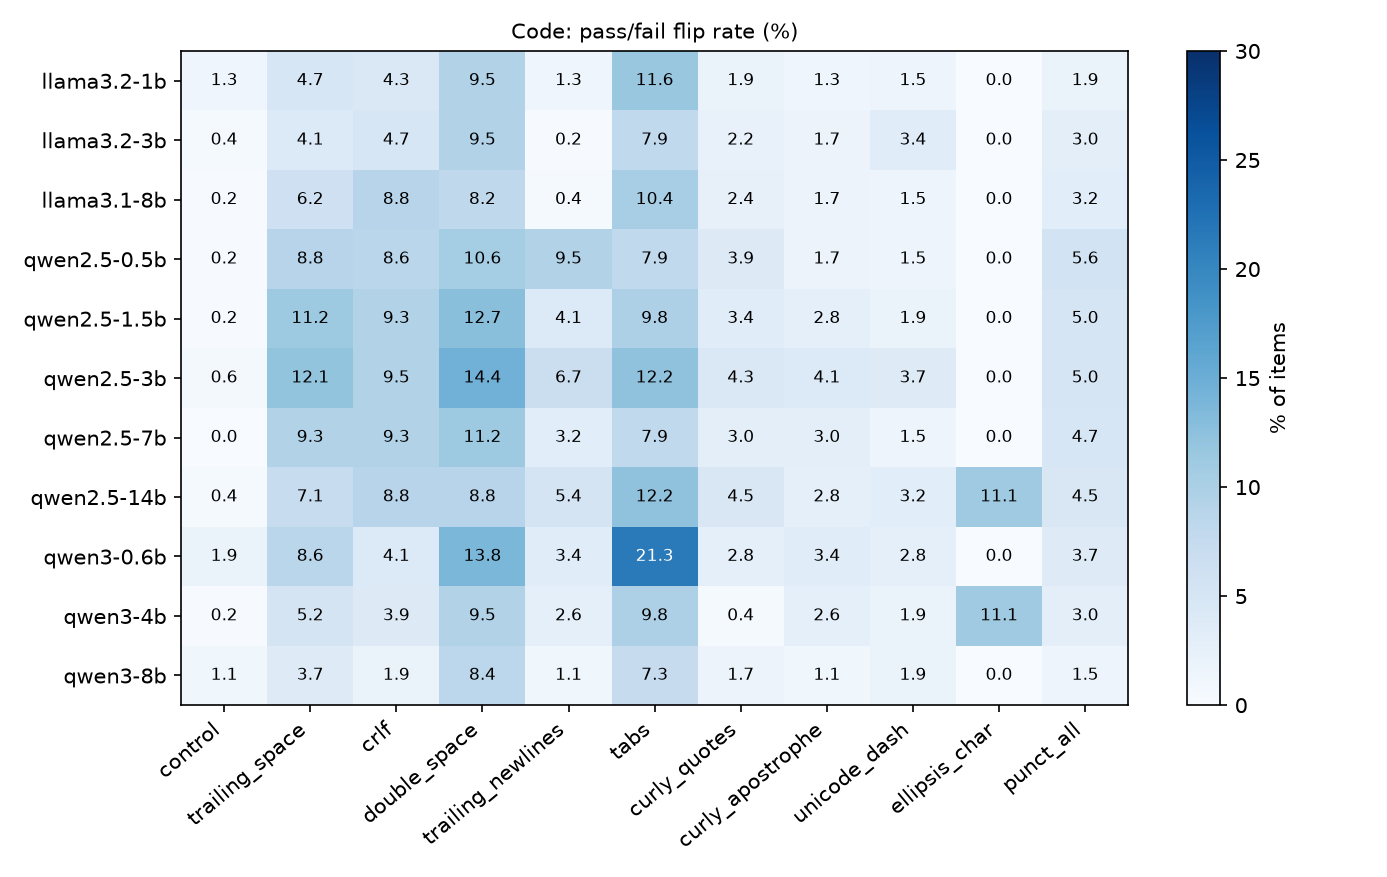
\includegraphics[width=0.8\linewidth]{figures/heat_code_flip.png}
    \caption{Code pass/fail flip rate (\%) per model and edit, pooled over \humaneval and \mbpp. Whitespace edits produce the largest functional changes across models. The 11.1\% \cond{ellipsis_char} cells correspond to a single program out of 9.}
    \label{fig:heat_code}
\end{figure}
